\chapter{Uma revisão sobre teste sistêmico}
%\addcontentsline{toc}{chapter}{Uma revisão do estado da arte em teste sistêmico, estrutural e funcional}

\section{Desafios no teste e validação de sistemas}

Conforme a literatura acadêmica \citep{jutman2014high} e também como prática da industria, o teste sistêmico tem de ser feito não somente após a manufatura, mas também para validação do sistema assim como no restante de seu ciclo de vida para manutenção e no diagnóstico dos retornos de campo. 

A complexidade destes sistemas requer - e ao mesmo tempo limita - a aplicação de uma abordagem de \textit{dividir para conquistar}. E é essencial realizar teste e diagnóstico de todos os componentes. Em caso  de encapsulamentos caros, a confiabilidade é um pouco maior, já que pra estes componentes existem políticas de \textit{Known Good Dies} (KGD)\footnote{Os circuitos são todos testados na própria fábrica, ainda nos waffers} e \textit{post-silicon validation} \citep{gilg1997known}. Mesmo assim isso somente não é suficiente já que suas interações com outros componentes do sistema também precisam ser validadas. Além disso, a integração e interação dos sistemas com o mundo real requerem o teste de propriedades não-funcionais como consumo de energia, desempenho térmico, e robustez sob diversas condições ambientais \citep{mitra2010post,ko2008distributed, jutman2014high}.

\section{Teste e diagnóstico no processo produtivo}

Dependendo da tecnologia utilizada, placas de circuito impresso podem ou não ser reparáveis. Independente disso, o dispositivo defeituoso precisa ser identificado e o diagnóstico é essencial tanto para o reparo quando para melhorias do processo produtivo \citep{ye2013board}. Se o reparo não é possível nas tecnologias avançadas, o diagnóstico ainda é necessário para compreender o problema e melhorar a produção. Pelas mesmas razões, \textit{SoCs} de sistemas defeituosos acabam também sujeitos a diagnósticos de falha \citep{tang2007analyzing, jutman2014high}.

\section{Diagnóstico na manutenção e retornos de campo}

Conforme \citet{jutman2014high}, a taxa de falha em campo pode ser interpretada como uma medida da dependência e da confiabilidade dos sistemas, e faz-se necessário que metas bem especificas das taxas de retorno sejam mantidas ou melhoradas. Isso também é importante no contexto de Controle de Qualidade e também para a alcançar certificações ISO.

O diagnóstico de sistemas eletrônicos é fundamental, e, em setores de aplicação como automotivo ou aeroespacial, a causa raiz de toda e qualquer falha sistêmica precisa ser esclarecida \citep{abelein2014non}. Em casos como esses, dois desafios precisam ser superados: Primeiramente, muitas falhas somente são observáveis sob condições específicas de operação, podendo desaparecer após a desmontagem do sistema (Jutman et al.,2014). 

Estes casos de \textit{Falha Não Encontrada} (ou em inglês, \textit{"No Failure Found"} ou NFF) acabam tornando-se caros e também introduzem riscos para outros produtos \citep{conroy2005practical}. Em segundo lugar, o OEM - \textit{Original Equipment Manufacturer}, como por exemplo um fabricante de veículos, depende de uma grande cadeia de fornecedores, e a identificação de falhas requer a colaboração de muitos parceiros (Figura 1-a). Segundo \citet{jutman2014high}, se as PCIs e circuitos integrados oferecerem uma boa capacidade de auto-diagnostico para o OEM, isso ajudaria a encurtar o processo de diagnóstico (Figura 1-b), além de poder ser usado sob condições típicas de operação para reduzir os NFF antes da desmontagem do sistema. Os dados coletados beneficiariam não só o OEM como também todos os membros da cadeia produtiva \citep{cook2014diagnosis}.
    \begin{figure}
        \centering
        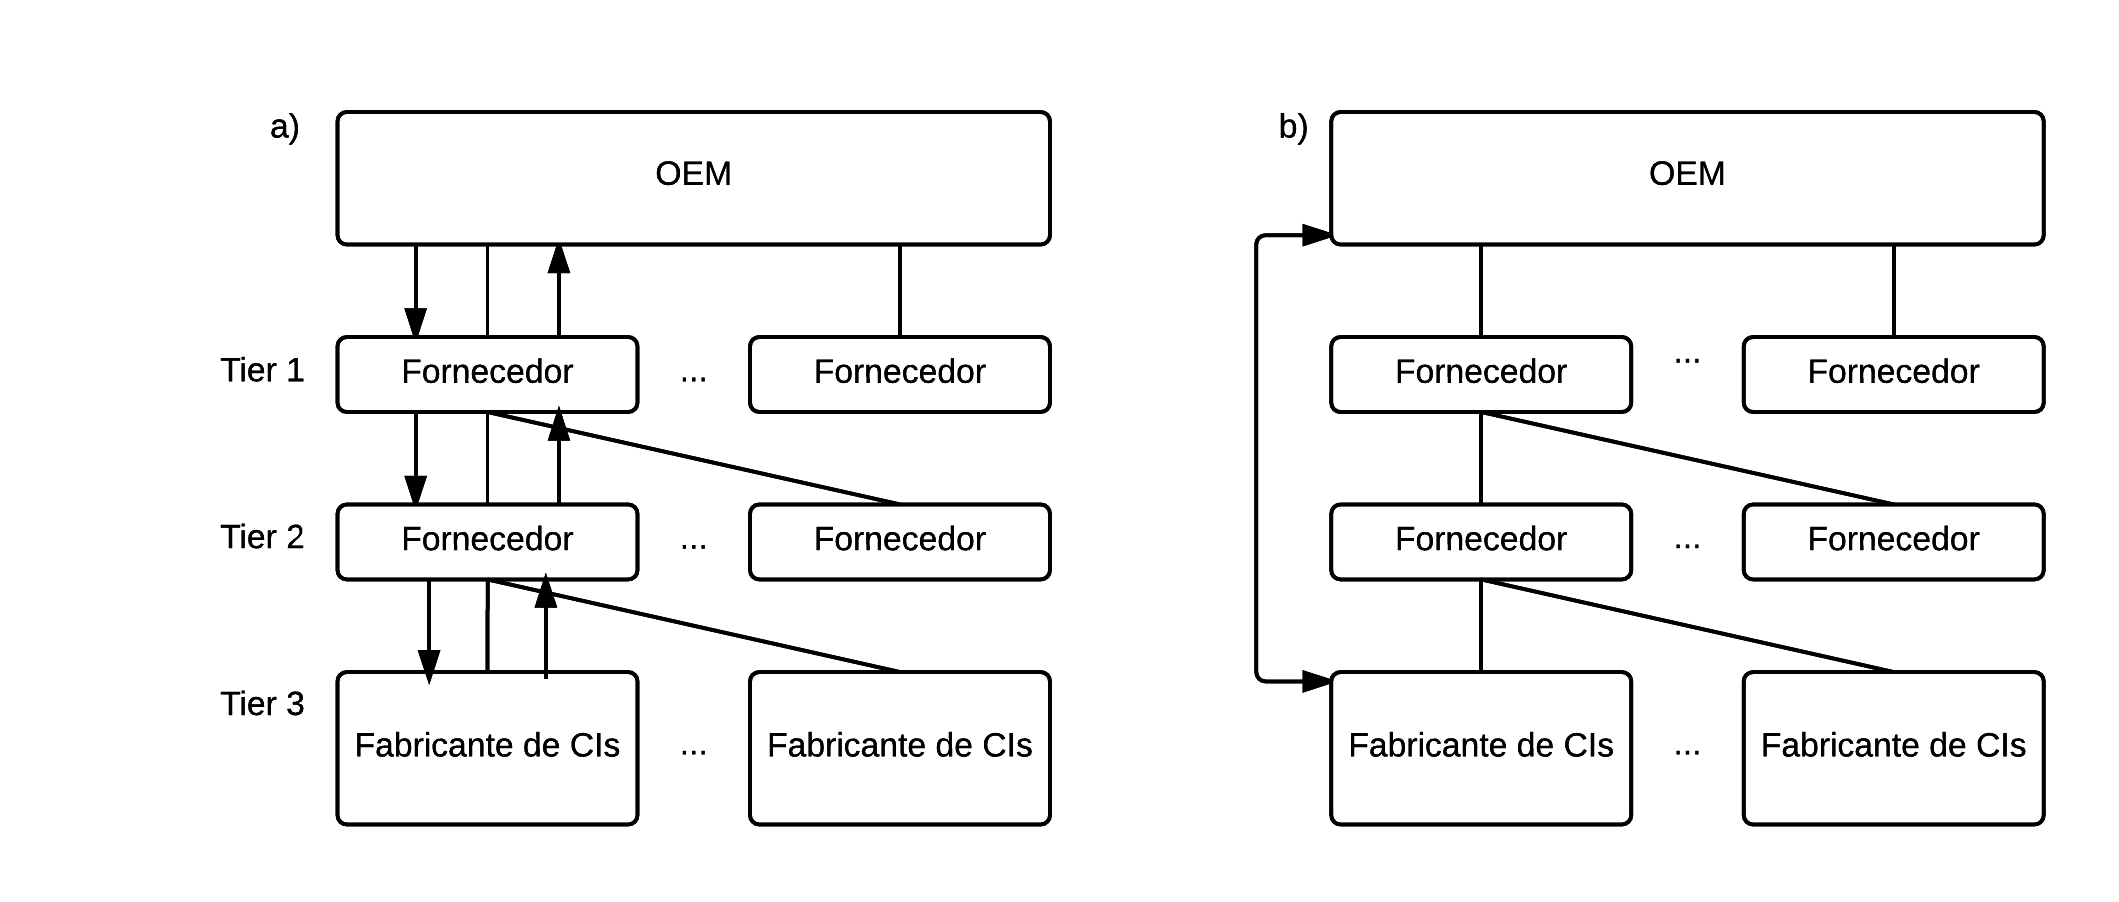
\includegraphics[width=.8\linewidth]{oem}
        \label{fig:supplychain}
        \caption{Diagnóstico do sistema no decorrer da cadeia de fornecedores. Adaptado de Jutman (2014)}
    \end{figure}
Dados de teste também podem ser coletados em campo \textit{on-line} e \textit{off-line} ou em concorrência ou não-concorrência. As respostas dos testes registradas em campo podem ajudar a diagnosticar os retornos de campo. Além do mais este tipo de teste é necessário para a checagem de funcionalidade de sistemas críticos (safety-critical systems).

O próximo capitulo descreve as práticas comuns, atuais desafios e técnicas avançadas em testes à nível de placa. E os capítulos seguintes especificam sobre testes estruturais e testes funcionais.
